\documentclass{entcs}
\usepackage{prentcsmacro}

\def\lastname{Carette, Chen, Choudhury, Rose, and Sabry}

%% Amr
%% words to remember :-)
%% sublime unfathomable
%% path categorical semantics
%% ---

\usepackage{bbold}
\usepackage{bussproofs}
\usepackage{keystroke}
\usepackage{comment}
\usepackage{tikz}
\usepackage[inline]{enumitem}
\usepackage{agda}

\newcommand{\byiso}[1]{{\leftrightarrow}{\langle} ~#1~ \rangle}
\newcommand{\unitepl}{\texttt{unitepl}}
\newcommand{\unitipl}{\texttt{unitipl}}
\newcommand{\unitepr}{\texttt{unitepr}}
\newcommand{\unitipr}{\texttt{unitipr}}
\newcommand{\swap}{\texttt{swap}}
\newcommand{\swapp}{\texttt{swapp}}
\newcommand{\assoclp}{\texttt{assoclp}}
\newcommand{\assocrp}{\texttt{assocrp}}
\newcommand{\unitetl}{\texttt{unitetl}}
\newcommand{\unititl}{\texttt{unititl}}
\newcommand{\unitetr}{\texttt{unitetr}}
\newcommand{\unititr}{\texttt{unititr}}
\newcommand{\swapt}{\texttt{swapt}}
\newcommand{\assoclt}{\texttt{assoclt}}
\newcommand{\assocrt}{\texttt{assocrt}}
\newcommand{\absorbr}{\texttt{absorbr}}
\newcommand{\absorbl}{\texttt{absorbl}}
\newcommand{\factorzr}{\texttt{factorzr}}
\newcommand{\factorzl}{\texttt{factorzl}}
\newcommand{\factor}{\texttt{factor}}
\newcommand{\distl}{\texttt{distl}}
\newcommand{\dist}{\texttt{dist}}
\newcommand{\factorl}{\texttt{factorl}}
\newcommand{\id}{\texttt{id}}
\newcommand{\compc}[2]{#1 \circ #2}
\newcommand{\compcc}[2]{#1 \bullet #2}
\newcommand{\respcomp}[2]{#1 \odot #2}

\newcommand{\Typ}{\mathbf{Type}}
\newcommand{\alt}{~\mid~}
\newcommand{\patht}[1]{\textsc{PATHS}(#1,#1)}
\newcommand{\fpatht}[1]{\textsc{FREEPATHS}(#1,\Box)}
\newcommand{\fpathp}[2]{\textsc{freepath}~#1~#2}
\newcommand{\pathind}[2]{\textsc{pathind}~#1~#2}
\newcommand{\invc}[1]{!\;#1}
\newcommand{\evalone}[2]{eval(#1,#2)}
\newcommand{\evalbone}[2]{evalB(#1,#2)}
\newcommand{\reflp}{\textsc{refl}}
\newcommand{\notp}{\textsc{not}}
\newcommand{\gluep}{\textsc{glue}}
\newcommand{\reflh}{\mathit{refl}_{\sim}}
\newcommand{\symh}[1]{\mathit{sym}_{\sim}~#1}
\newcommand{\transh}[2]{\mathit{trans}_{\sim}~#1~#2}
\newcommand{\reflq}{\mathit{refl}_{\simeq}}
\newcommand{\symq}[1]{\mathit{sym}_{\simeq}~#1}
\newcommand{\transq}[2]{\mathit{trans}_{\simeq}~#1~#2}
\newcommand{\isequiv}[1]{\mathit{isequiv}(#1)}
\newcommand{\idc}{\mathit{id}_{\boolt}}
\newcommand{\swapc}{\mathit{swap}_{\boolt}}
\newcommand{\assocc}{\mathit{assoc}}
\newcommand{\invl}{\mathit{invl}}
\newcommand{\invr}{\mathit{invr}}
\newcommand{\invinv}{\mathit{inv}^2}
\newcommand{\idlc}{\mathit{idl}}
\newcommand{\idrc}{\mathit{idr}}
\newcommand{\swapswap}{\swapc^2}
\newcommand{\compsim}{\compc_{\isotwo}}
\newcommand{\iso}{\leftrightarrow}
\newcommand{\isotwo}{\Leftrightarrow}
\newcommand{\piso}{\multimapdotbothB~~}
\newcommand{\zt}{\mathbb{0}}
\newcommand{\ot}{\mathbb{1}}
\newcommand{\bt}{\mathbb{2}}
\newcommand{\fc}{\mathit{false}}
\newcommand{\tc}{\mathit{true}}
\newcommand{\boolt}{\mathbb{B}}
\newcommand{\univ}{\mathcal{U}}
\newcommand{\uzero}{\mathcal{U}_0}
\newcommand{\uone}{\mathcal{U}_1}
\newcommand{\Rule}[2]{
\makebox{
$\displaystyle
\frac{\begin{array}{l}#1\\\end{array}}
{\begin{array}{l}#2\\\end{array}}$}}
\newcommand{\proves}{\vdash}
\newcommand{\jdgg}[3]{#1 \proves #2 : #3}
\newcommand{\jdg}[2]{\proves #1 : #2}
\newcommand{\jdge}[3]{\proves #1 = #2 : #3}
%% codes
%% denotations

\newcommand{\amr}[1]{\fbox{\begin{minipage}{0.8\textwidth}\color{red}{Amr says: {#1}}\end{minipage}}}
\newcommand{\jacques}[1]{\fbox{\begin{minipage}{0.8\textwidth}\color{red}{Jacques says: {#1}}\end{minipage}}}

%%%%%%%%%%%%%%%%%%%%%%%%%%%%%%%%%%%%%%%%%%%%%%%%%%%%%%%%%%%%%%%%%%%%%%%%%%%%%%
\begin{document}

\begin{frontmatter}
\title{From Reversible Programs to \\ Univalent Universes and Back}
\author{Jacques Carette}
\address{McMaster University}
\author{Chao-Hong Chen}
\address{Indiana University}
\author{Vikraman Choudhury}
\author{Robert Rose}
\author{Amr Sabry}
\address{Indiana University}

\begin{abstract}
  We establish a close connection between a reversible programming language
  based on type isomorphisms and a formally presented univalent universe. The
  correspondence relates combinators witnessing type isomorphisms in the
  programming language to paths in the univalent universe and combinator
  optimizations in the programming language to 2-paths in the univalent
  universe. The result suggests a simple computational interpretation of paths
  and of univalence in terms of familiar programming constructs whenever the
  universe in question is computable.
\end{abstract}

\end{frontmatter}

%%%%%%%%%%%%%%%%%%%%%%%%%%%%%%%%%%%%%%%%%%%%%%%%%%%%%%%%%%%%%%%%%%%%%%%%%%%%%%
\section{Introduction}

The proceedings of the 2012 Symposium on Principles of Programming
Languages~\cite{Field:2012:2103656} included two apparently unrelated papers:
\emph{Information Effects} by James and Sabry and \emph{Canonicity for
  2-dimensional type theory} by Licata and Harper. The first paper, motivated by
the physical nature of
computation~\cite{Landauer:1961,PhysRevA.32.3266,Toffoli:1980,bennett1985fundamental,Frank:1999:REC:930275},
proposed, among other results, a reversible language $\Pi$ in which every
program is a type isomorphism. The second paper, motivated by the connections
between homotopy theory and type theory~\cite{vv06,hottbook}, proposed a
judgmental formulation of intensional dependent type theory with a
twice-iterated identity type. During the presentations and ensuing discussions
at the conference, it became apparent, at an intuitive and informal level, that
the two papers had strong similarities. Formalizing the precise connection was
far from obvious, however.

In this paper we report on a formal connection between appropriately formulated
reversible languages on one hand and univalent universes on the other. In the
next section, we give a rational reconstruction of $\Pi$ focusing on a small
``featherweight'' fragment. In Sec.~\ref{sec:univalent}, we review
\emph{univalent fibrations} which allow us to give formal presentations of
``small'' univalent universes. In Sec.~\ref{sec:connection} we state and prove
the formal connection between the systems presented in the preceding two
sections. Sec.~\ref{sec:conclusion} puts our work in a larger context, discusses
related and future work, and concludes.

%%%%%%%%%%%%%%%%%%%%%%%%%%%%%%%%%%%%%%%%%%%%%%%%%%%%%%%%%%%%%%%%%%%%%%%%%%%%%%
\section{A Simple Reversible Programming Language}

Starting from the physical principle of ``conservation of
information''~\cite{Hey:1999:FCE:304763,fredkin1982conservative}, James and
Sabry~\cite{James:2012:IE:2103656.2103667} propose a family of programming
languages $\Pi$ in which computation preserve information. Technically,
computations are \emph{type isomorphisms} which, at least in the case of finite
types, clearly preserve entropy in the information-theoretic
sense~\cite{James:2012:IE:2103656.2103667}. We will identify a ``featherweight''
version of $\Pi$ to use in our formal development.  But first we illustrate the
general flavor of the family of languages with some examples.

%%%%%
\subsection{Examples}

\jacques{Example 1: using the combinators from pi-dual, some an equational
derivation in type theory (which?), in equational-derivation style.  Point out
that reading ``down'' the justifications is a $\Pi$ program which is also a
constructive proof of the equivalence of the types.  As it is reversible, we
can also read the reverse program by reading ``up''.}

{\small
\[\def\arraystretch{1.2}\begin{array}{rcl}
\AgdaFunction{controlled} &:& \forall a.~ (a \leftrightarrow a) \rightarrow 
                              (\bt \otimes a \leftrightarrow \bt \otimes a) \\
\AgdaFunction{controlled}~\AgdaFunction{f} &=& 
      \bt \otimes a \\
&& \qquad\byiso{\AgdaFunction{unfoldBool} \otimes \AgdaFunction{id}} \\
&& (\ot \oplus \ot) \otimes a \\
&& \qquad\byiso{\AgdaFunction{dist}} \\
&& (\ot \otimes a) \oplus (\ot \otimes a) \\
&& \qquad\byiso{\AgdaFunction{id} \oplus (\AgdaFunction{id} \otimes \AgdaFunction{f})} \\
&& (\ot \otimes a) \oplus (\ot \otimes a) \\
&& \qquad\byiso{\AgdaFunction{factor}} \\
&& (\ot \oplus \ot) \otimes a \\
&& \qquad\byiso{\AgdaFunction{foldBool} \otimes \AgdaFunction{id}} \\
&& \bt \otimes a \\
\\ 
\AgdaFunction{not}~\AgdaFunction{not₁}~\AgdaFunction{not₂}~\AgdaFunction{not₃} &:& 
     \bt \leftrightarrow \bt \\
\AgdaFunction{not} &=& 
  \AgdaFunction{unfoldBool} \odot \AgdaFunction{swap₊} \odot \AgdaFunction{foldBool} \\
\AgdaFunction{not₁} &=& 
  \AgdaFunction{id} \odot \AgdaFunction{not} \\
\AgdaFunction{not₂} &=& 
  \AgdaFunction{not} \odot \AgdaFunction{not} \odot \AgdaFunction{not} \\
\AgdaFunction{not₃} &=& 
  \AgdaFunction{uniti⋆} \odot \AgdaFunction{swap⋆} \odot
                        (\AgdaFunction{not} \otimes \AgdaFunction{id}) \odot
                        \AgdaFunction{swap⋆} \odot
                        \AgdaFunction{unite⋆} \\
\\ 
\AgdaFunction{not} &:& \bt \leftrightarrow \bt \\
\AgdaFunction{not} &=& 
  \AgdaFunction{unfoldBool} \odot \AgdaFunction{swap₊} \odot \AgdaFunction{foldBool} \\
\\ 
\AgdaFunction{cnot} &:& \bt \otimes \bt \leftrightarrow \bt \otimes \bt \\
\AgdaFunction{cnot} &=& \AgdaFunction{controlled}~\AgdaFunction{not} \\
\\ 
\AgdaFunction{toffoli} &:& \bt \otimes (\bt \otimes \bt)
                           \leftrightarrow  \bt \otimes (\bt \otimes \bt) \\
\AgdaFunction{toffoli} &=& \AgdaFunction{controlled}~\AgdaFunction{cnot}
\end{array}\]}


\jacques{Example 2: like example 1, but this time at the next level (i.e. a
program equivalence).  Same remark old.  Refer to Shulmann notes, and point out
that such equational proofs at this level can actually be interpreted in appropriate
categories as commutative diagrams.}

\jacques{Refer to some Sabry et al. papers regarding Toffoli gates.}

% \begin{comment}
% In this paper we will
% identify a ``featherweight'' representative to use for the formal
% development. But first, we illustrate the flavor of the family of languages with
% some examples written in a Haskell syntax. First consider the following program:

% {\footnotesize
% \begin{verbatim}
% addSub1 :: (Int, Int) :<=> (Int, Int)
% addSub1 = CommuteTimes
%       :.: (UnfoldN :*: Id)
%       :.: Distribute
%       :.: (Id :+: CommuteTimes)
%       :.: Factor
%       :.: (FoldN :*: Id)
% \end{verbatim}}
% %
% \noindent which takes a pair of natural numbers and processes them as follows depending on
% whether the second number is 0 or not. If the second number is 0, the evaluation
% proceeds as follows:
% $(n,0) \mapsto (0,n) \mapsto (\mathit{inj}_1(),n) \mapsto \mathit{inj}_1((),n)
% \mapsto \mathit{inj}_1((),n) \mapsto (\mathit{inj}_1(),n) \mapsto (0,n)$. If the
% second number is $\mathit{suc}~m$, the evaluation proceeds as follows:
% $(n, \mathit{suc}~m) \mapsto (\mathit{suc}~m,n) \mapsto (\mathit{inj}_2m,n)
% \mapsto \mathit{inj}_2(m,n) \mapsto \mathit{inj}_2(n,m) \mapsto
% (\mathit{inj}_2n,m) \mapsto (\mathit{suc}~n,m)$. In summary, repeated
% applications of this program would increment the first number and decrement the
% second number maintaining the sum at all times. When the second number reaches
% 0, the numbers are swapped.

% As another example, consider the following expressions culminating with the
% implementation of the Toffoli gate, which is universal for combinational
% circuits. We have two implementations of simple boolean negation: a direct one
% and a more convoluted one. These two implementations are ``equivalent'' in the
% sense to be explained below. The expression \verb|cond| is the main reversible
% control flow mechanism: it allows for the conditional execution of one of two
% branches but retains the choice of which branch was executed. This mechanism can
% be used twice to implement the Toffoli gate, which performs a conditional
% negation on one bit if two other bits are both true:

% {\footnotesize
% \begin{verbatim}
% inot :: Bool :<=> Bool
% inot = CommutePlus

% inot2 :: Bool :<=> Bool
% inot2 = UnitTimesI
%     :.: CommuteTimes
%     :.: (CommutePlus :*: Id)
%     :.: CommuteTimes
%     :.: UnitTimesE

% cond :: (a :<=> b) -> (a :<=> b) -> ((Bool, a) :<=> (Bool, b))
% cond f g = Distribute
%        :.: ((Id :*: f) :+: (Id :*: g))
%        :.: Factor

% controlled :: (a :<=> a) -> ((Bool, a) :<=> (Bool, a))
% controlled f = cond f Id

% cnot :: (Bool, Bool) :<=> (Bool, Bool)
% cnot = controlled inot

% toffoli :: ((Bool,Bool),Bool) :<=> ((Bool,Bool),Bool)
% toffoli = AssocTimesR :.: controlled cnot :.: AssocTimesL
% \end{verbatim}}

% Although writing circuits using the raw syntax for combinators above is tedious,
% the examples illustrate the programming language nature of this family of $\Pi$
% languages. In other work, one can find a compiler from a conventional functional
% language to circuits~\cite{James:2012:IE:2103656.2103667}, a systematic
% technique to translate abstract machines to $\Pi$~\cite{rc2012}, and a
% Haskell-like surface language~\cite{theseus} which can ease writing
% programs. All that reinforces the claim that this is a practical approach to
% reversible programming.

% The raw syntax for combinators has, however, a significant benefit: it allows
% algebraic manipulation of the programs using a second level of combinators. As
% an example it is possible to show the the two implementations of boolean
% negation are equivalent as follows:

% {\footnotesize
% \begin{verbatim}
% negOpt :: inot2 :<===> inot
% negOpt = (Id :>: AssocLeftEquiv)
%     :..: (Id :>: (SlideCommuteTimes :>: Id))
%     :..: (Id :>: AssocRightEquiv)
%     :..: (Id :>: (Id :>: AssocLeftEquiv))
%     :..: (Id :>: (Id :>: (InvInvEquivId :>: Id)))
%     :..: (Id :>: (Id :>: IdElimL))
%     :..: AssocLeftEquiv
%     :..: (SlideUnitI :>: Id)
%     :..: AssocRightEquiv
%     :..: (Id :>: InvInvEquivId)
%     :..: IdElimR
% \end{verbatim}}
% %
% \noindent This program, which can be thought of as an optimization or a proof,
% relates the two implementations of boolean negation via a series of elementary
% optimizations of which the following are the most interesting:

% {\footnotesize
% \begin{verbatim}
% AssocLeftEquiv    ::           (c1 :.: (c2 :.: c3)) :<===> ((c1 :.: c2) :.: c3)
% SlideCommuteTimes :: (CommuteTimes :.: (c1 :*: c2)) :<===> ((c2 :*: c1) :.: CommuteTimes)
% IdElimL           ::                     (Id :.: c) :<===> c
% SlideUnitI        ::   (UnitTimesI :.: (c1 :*: c2)) :<===> (c2 :.: UnitTimesI)
% \end{verbatim}}

% \end{comment}

%%%%%
\subsection{$\Pi_{\mathbb{2}}$}

We present a small $\Pi$-based language which we will use in the formalization
in the rest of the paper. The restriction of $\Pi$ to the case of just booleans
is the following:

\[\begin{array}{rcl}
\tau &::=& \bt \\
\\
v &::=& \begin{array}[t]{lrcl}
                    & \fc &:& \bt \\
              \alt & \tc &:& \bt
               \end{array} \\
\\
c &::=& \begin{array}[t]{llcl}
              & \id &:& \tau \iso \tau \\
               \alt & \swap &:& \bt \iso \bt \\
               \alt & ! &:& (\tau_1 \iso \tau_2) \to (\tau_2 \iso \tau_1) \\
               \alt & \circ &:& (\tau_1 \iso \tau_2) \to (\tau_2 \iso \tau_3) \to (\tau_1 \iso \tau_3)
               \end{array} \\
\\
\alpha &::=& \begin{array}[t]{lrcl}
               & \id &:& c \isotwo c \\
            \alt & \idlc &:& \compc{\id}{c} \isotwo c \\
            \alt & \idrc &:& \compc{c}{\id} \isotwo c \\
            \alt & \invl &:& \compc{c\;}{\;\invc{c}} \isotwo \id \\
            \alt & \invr &:& \compc{\invc{c}}{c} \isotwo \id \\
            \alt & \rho &:& \swap \circ \swap \isotwo \id \\
            \alt & \assocc &:& \compc{(\compc{c_1}{c_2})}{c_3} \isotwo \compc{c_1}{(\compc{c_2}{c_3})} \\
            \alt & \odot &:& (c_1 \isotwo c_1') \to (c_2 \isotwo c_2') \to (\compc{c_1}{c_2} \isotwo \compc{c_1'}{c_2'}) \\
            \alt & !! &:& (c_1 \isotwo c_2) \to (c_2 \isotwo c_1) \\
            \alt & \bullet &:& (c_1 \isotwo c_2) \to (c_2 \isotwo c_3) \to (c_1 \isotwo c_3)
             \end{array}
\end{array}\]

Canonical forms: given a level 1 program p, the level 2 combinators are
complete; they can transform p to either id or not:
\begin{verbatim}
cmpl2-lem : (p : B <->1 B) -> (p <->2 id) + (p <->2 not)
\end{verbatim}

%%%%%%%%%%%%%%%%%%%%%%%%%%%%%%%%%%%%%%%%%%%%%%%%%%%%%%%%%%%%%%%%%%%%%%%%%%%%%%
\section{Univalent Fibrations}
\label{sec:univalent}

We will consider a general statement of \emph{univalence} for type families. We
start with a some preliminaries. Fig.~\ref{fig:fib} depicts a type family
$P : A \rightarrow \mathcal{U}$ mapping each point $x : A$ to a space $P(x)$. As
everything is continuous, we expect this type family to respect identities. In
other words if $x:A$ and $y:A$ are identified using a path $x \equiv y$, it must
be the case that the spaces $P(x)$ and $P(y)$ become equivalent
$P(x) \simeq P(y)$ as a consequence. Generally speaking, there is no reason to
expect that the spaces $x \equiv y$ and $P(x) \simeq P(y)$ to be themselves
equivalent for all $x$ and $y$. And indeed they are most frequently not
equivalent. In the rare cases in which they are equivalent, the fibration is a
\emph{univalent fibration}.

\begin{figure}
\begin{tabular}{c@{\qquad\qquad}c}
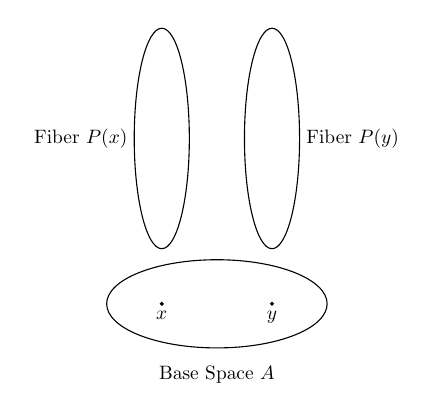
\begin{tikzpicture}[scale=0.7,every node/.style={scale=0.7}]]
  \draw (0,-5) ellipse (2cm and 0.8cm);
  \node[below] at (0,-6) {Base Space $A$};
  \draw[fill] (-1,-5) circle [radius=0.025];
  \node[below] at (-1,-5) {$x$};
  \draw[fill] (1,-5) circle [radius=0.025];
  \node[below] at (1,-5) {$y$};
  \draw (-1,-2) ellipse (0.5cm and 2cm);
  \node[left] at (-1.5,-2) {Fiber $P(x)$};
  \draw (1,-2) ellipse (0.5cm and 2cm);
  \node[right] at (1.5,-2) {Fiber $P(y)$};
\end{tikzpicture}
&
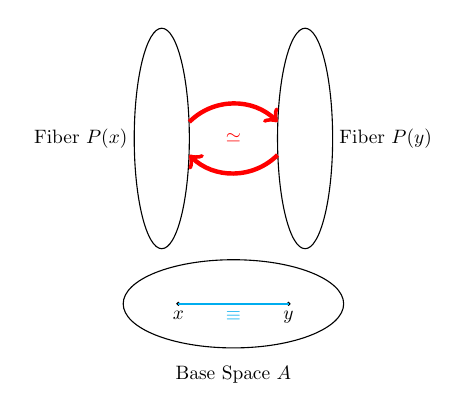
\begin{tikzpicture}[scale=0.7,every node/.style={scale=0.7}]]
  \draw (0,-5) ellipse (2cm and 0.8cm);
  \node[below] at (0,-6) {Base Space $A$};
  \draw[fill] (-1,-5) circle [radius=0.025];
  \node[below] at (-1,-5) {$x$};
  \draw[fill] (1,-5) circle [radius=0.025];
  \node[below] at (1,-5) {$y$};
  \draw (-1.3,-2) ellipse (0.5cm and 2cm);
  \node[left] at (-1.8,-2) {Fiber $P(x)$};
  \draw (1.3,-2) ellipse (0.5cm and 2cm);
  \node[right] at (1.8,-2) {Fiber $P(y)$};
  \draw[below,cyan,thick] (-1,-5) -- (1,-5);
  \node[below,cyan,thick] at (0,-5) {$\equiv$};
  \draw[->,red,ultra thick] (-0.8,-1.7) to [out=45, in=135] (0.8,-1.7);
  \draw[->,red,ultra thick] (0.8,-2.3) to [out=-135, in=-45] (-0.8,-2.3);
  \node[red,ultra thick] at (0,-2) {$\simeq$};
\end{tikzpicture}
\end{tabular}
\caption{\label{fig:fib}(left) Type family $P : A \rightarrow \mathcal{U}$ as a
  fibration with total space $\Sigma_{(x:A)} P(x)$; (right) a path $x \equiv y$
  in the base space induces an equivalence between the spaces $P(x)$ and $P(y)$}
\end{figure}

As two simple examples of non-univalent fibrations consider
$P : \mathbb{1} \rightarrow \mathbb{U}$ defined as $P = \lambda\_.\mathbb{2}$
and $Q : \mathbb{2} \rightarrow \mathbb{U}$ defined as
$Q = \lambda \_. \mathbb{1}$ illustrated below:

\begin{tabular}{c@{\qquad\qquad}c}
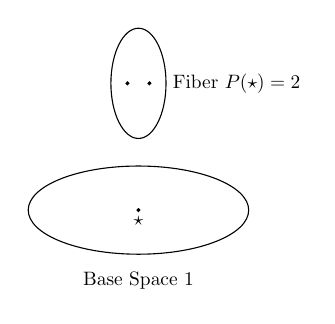
\begin{tikzpicture}[scale=0.7,every node/.style={scale=0.7}]]
  \draw (0,-5) ellipse (2cm and 0.8cm);
  \node[below] at (0,-6) {Base Space $\mathbb{1}$};
  \draw[fill] (0,-5) circle [radius=0.025];
  \node[below] at (0,-5) {$\star$};
  \draw (0,-2.7) ellipse (0.5cm and 1cm);
  \node[right] at (0.5,-2.7) {Fiber $P(\star) = \mathbb{2}$};
  \draw[fill] (-0.2,-2.7) circle [radius=0.025];
  \draw[fill] (0.2,-2.7) circle [radius=0.025];
\end{tikzpicture}
&
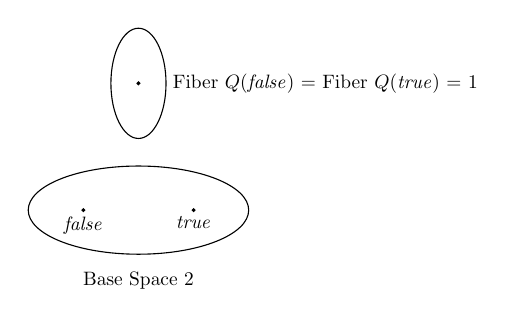
\begin{tikzpicture}[scale=0.7,every node/.style={scale=0.7}]]
  \draw (0,-5) ellipse (2cm and 0.8cm);
  \node[below] at (0,-6) {Base Space $\mathbb{2}$};
  \draw[fill] (-1,-5) circle [radius=0.025];
  \node[below] at (-1,-5) {$\fc$};
  \draw[fill] (1,-5) circle [radius=0.025];
  \node[below] at (1,-5) {$\tc$};
  \draw (0,-2.7) ellipse (0.5cm and 1cm);
  \node[right] at (0.5,-2.7) {Fiber $Q(\fc)$ = Fiber $Q(\tc)$ = $\mathbb{1}$};
  \draw[fill] (0,-2.7) circle [radius=0.025];
\end{tikzpicture}
\end{tabular}

\medskip\noindent The identity function and boolean negation induce two distinct
equivalences in the space $P(\star) = \mathbb{2} \simeq \mathbb{2} =
P(\star)$. As there is only one path $\star \equiv \star$ in the base space, the
fibration $P$ is not univalent. Similarly, there is one equivalence
$Q(\fc) = \mathbb{1} \simeq \mathbb{1} = Q(\tc)$ but this certainly does not
induce a path $\fc \equiv \tc$. As the examples illustrate there is a delicate
balance required for the fibration to be univalent; otherwise some distinct
equivalences would be identified (like for $P$) or distinct points in the base
space would be identified (like for $Q$).

An example of a univalent fibration is $P : \mathbb{2} \rightarrow \mathbb{U}$
defined as $P(\fc) = \mathbb{0}$ and $P(\tc) = \mathbb{1}$ illustrated below:

\bigskip
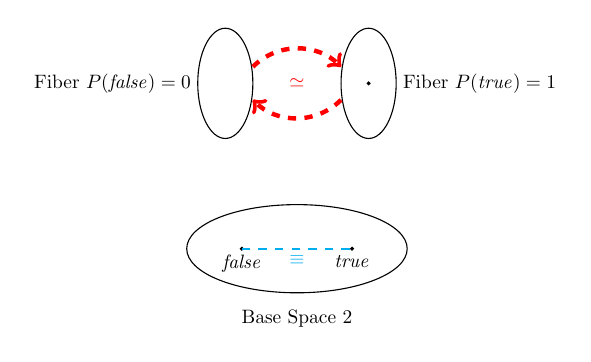
\begin{tikzpicture}[scale=0.7,every node/.style={scale=0.7}]]
  \draw (0,-5) ellipse (2cm and 0.8cm);
  \node[below] at (0,-6) {Base Space $\mathbb{2}$};
  \draw[fill] (-1,-5) circle [radius=0.025];
  \node[below] at (-1,-5) {$\fc$};
  \draw[fill] (1,-5) circle [radius=0.025];
  \node[below] at (1,-5) {$\tc$};
  \draw (-1.3,-2) ellipse (0.5cm and 1cm);
  \node[left] at (-1.8,-2) {Fiber $P(\fc) = \mathbb{0}$};
  \draw (1.3,-2) ellipse (0.5cm and 1cm);
  \draw[fill] (1.3,-2) circle [radius=0.025];
  \node[right] at (1.8,-2) {Fiber $P(\tc) = \mathbb{1}$};
  \draw[below,cyan,dashed,thick] (-1,-5) -- (1,-5);
  \node[below,cyan,dashed,thick] at (0,-5) {$\equiv$};
  \draw[->,red,dashed,ultra thick] (-0.8,-1.7) to [out=45, in=135] (0.8,-1.7);
  \draw[->,red,dashed,ultra thick] (0.8,-2.3) to [out=-135, in=-45] (-0.8,-2.3);
  \node[red,ultra thick] at (0,-2) {$\simeq$};
\end{tikzpicture}

\medskip\noindent In this case, the space of equivalences
$P(\fc) = \mathbb{0} \simeq \mathbb{1} = P(\tc)$ is empty and so is the space of
paths $\fc \equiv \tc$ and hence these two spaces are vacuously equivalent.

%%%
\subsection{A Special Class}

Instead of guessing, there is a special class of univalent fibrations:
\[\begin{array}{rcl}
\{F\} &:& \Sigma_{A:\mathcal{U}} \| F \equiv A \| \rightarrow \mathcal{U} \\
\{F\}(A,|p|) &=& A
\end{array}\]

This construction is always a univalent fibration~\cite{XXX}. We can understand
the basic idea as follows. Take two points $(A,|p|)$ and $(B,|q|)$ in the base
space. We want to compare the space $A \simeq B$ with the space
$(A,|p|) \equiv (B,|q|)$.  In one direction, we have $p : F \equiv A$ and
$q : F \equiv B$ and hence $A \equiv B$ and by univalence $A \simeq B$. In the
other direction \ldots

Also explain base space has higher paths \ldots

\begin{verbatim}
Thm: Let P : Type -> Type such that for all X : Type, P(X)
is a proposition. Then Σ(X,P) is the base of a univalent
fibration.

Furthermore, we have that *all* univalent fibrations
over Type arise this way. We don't need this fact directly,
but it may help in the explanation. (It's certainly cleaner
than making the connection to classifying bundles in
geometry).

Here are some more examples.

is-prop : Type -> Type has the property that is-prop(X)
is a proposition for all types X. So Σ(X , is-prop) is
the base of a univalent fibration. In other words, this
is the subuniverse consisting of all and only propositions.

is-set : Type -> Type has the property that is-set(X)
is a proposition for all types X. So Σ(X , is-set) is
the base of a univalent fibration. In other words, this
is the subuniverse consisting of all and only sets.

is-1-type : Type -> Type has the property that
is-1-type(X) is a proposition for all types X. So
Σ(X , is-1-type) is the base of a univalent fibration.
In other words, this is the subuniverse consisting of all
and only 1-types. (Externally, these are the 1-groupoids
embedded in inf-groupoids.)

But here's a summary of what I wrote last week, which
I think should suffice for this project. Designating a
collection of types as a univalent universe boils down
to defining a mere predicate on the universe. One approach
to defining such a predicate is to generate a set of
names and an interpretation El (a type family over
these names), and ask that the disjunction "is equal
to the interpretation of a name" be exclusive (i.e.,
a proposition). This last step requires that the set
of names be representatives of distinct normal forms.
Repackage these data --- the collection of types, their
names, and the proof that the predicate on the universe
is a proposition -- as a semantic object admitting
various presentations, which when computable, can be
called a "reversible programming language".

Because "the proof that the predicate on the universe
is a proposition" (and univalence), we naturally get a
family of equivalences arising.  At various levels.
When reflected syntactically, we get multiple
presentations of the same semantic object (where
'same' is really up to things 1 level up).  Because
all we can really talk about are equivalences, when
this syntax is interpreted as a programming language,
it is unavoidably reversible.

Right, the predicate being a proposition suffices
(and is necessary) to define an embedding into a
univalent universe.

(Univalence is used axiomatically, as is the rest of
the type theory, to define the universe. But you're
welcome to interpret ITT + univalence in simplicial
sets and forget about univalence altogether: the
univalent universe is a particular simplicial set
defined in classical set theory, as are the rest
of the subuniverses serving as denotational models.)

By "admitting various presentations", I mean
presentation in the sense of group presentation.
For example, the real functions on R^2 which are
symmetries of the square centered at the origin
can be viewed as the dihedral group on 8 elements:
but we're free to present this group in an infinite
number of ways. These presentations can be taken to
be syntax for a language. If a presentation has a
decidable word problem, and you have the algorithm,
then you could be said to have an operational
semantics, and so a programming language of a sort.
This is what, I take it, you and Amr did with Laplaza's
work on presenting free distributive categories
in the first place. There your semantic object is
the syntactic category of his theory of distributive
categories.

What using HoTT as a metatheory facilitates here is
the construction of models which admit presentations
of infinity-groupoids. (You could do it without HoTT.
But the results would likely be less general, say if
the work was done directly in simplicial sets or
cubical sets.) Using this approach, you have a lot
more options now for cooking up reversible PLs now;
just as many as you have decidable presentations of
inf-groupoids.

The 'exclusive disjunction' aspect of being a
proposition seems to have more content: it's a
sort of decidability / normal form property all
rolled into one.

Yes, I was struck by this too. At least insofar
as we continue with this style of defining predicates
on the universe to obtain the intended interpretation
of the types in a rev PL, it seems that a decidable
enumeration of normal forms of the types will already
be needed. But this doesn't seem like a huge constraint
to me; most of the action is at the level of the paths....

I guess that you assumed in "This last step requires
that the set of names be representatives of distinct
normal forms" that these were also complete?  That we
have a decidable enumeration of all normal forms?

I haven't said anything about an actual presentation
of the inf-groupoid which is the univalent universe
of finite types. You want Pi to do this work. So to
get started, we should define a function from the
BNF grammar corresponding to a syntax for a semiring
to the terms of that universe. As it stands, we
already know that those terms are reflected in Names,
so it would be sufficient to define that function
into Names. Ah, is this what you meant by "complete"?
Yes, we have a name for everything in the extension of
that predicate (by construction).

\end{verbatim}


That space {2} is a higher groupoid. Let's look at its objects; its 1-paths; its
2-paths etc.

Show Agda code

%%%%%%%%%%%%%%%%%%%%%%%%%%%%%%%%%%%%%%%%%%%%%%%%%%%%%%%%%%%%%%%%%%%%%%%%%%%%%%
\section{Correspondence}
\label{sec:connection}

In previous work, on $\Pi$ we noted a possible connection with HoTT:
\begin{quote}
  It is, therefore, at least plausible that a variant of HoTT based exclusively
  on reversible functions that directly correspond to equivalences would have
  better computational properties. Our current result is a step, albeit
  preliminary, in that direction as it only applies to finite
  types~\cite{Carette2016}.
\end{quote}
Formalizing, in a precise sense, the connection between reversible programs
based on combinators and paths in HoTT, as intuitive as it may seem, is however
difficult. Paths in HoTT come equipped with principles like the
``contractibility of singletons'', ``transport'', and ``path induction.'' None
of these principles seems to have any direct counterpart in the world of
reversible programming.

Soundness; completeness; etc.


%%%%%%%%%%%%%%%%%%%%%%%%%%%%%%%%%%%%%%%%%%%%%%%%%%%%%%%%%%%%%%%%%%%%%%%%%%%%%%
\section{Discussion, Related Work, and Conclusion}
\label{sec:conclusion}

\paragraph*{Reversible Languages.}
\noindent The practice of programming languages is replete with \emph{ad hoc}
instances of reversible computations: database transactions, mechanisms for data
provenance, checkpoints, stack and exception traces, logs, backups, rollback
recoveries, version control systems, reverse engineering, software transactional
memories, continuations, backtracking search, and multiple-level ``undo''
features in commercial applications. In the early nineties,
Baker~\cite{Baker:1992:LLL,Baker:1992:NFT} argued for a systematic, first-class,
treatment of reversibility. But intensive research in full-fledged reversible
models of computations and reversible programming languages was only sparked by
the discovery of deep connections between physics and
computation~\cite{Landauer:1961,PhysRevA.32.3266,Toffoli:1980,bennett1985fundamental,Frank:1999:REC:930275},
and by the potential for efficient quantum
computation~\cite{springerlink:10.1007/BF02650179}.

The early developments of reversible programming languages started with a
conventional programming language, e.g., an extended $\lambda$-calculus, and either
\begin{enumerate}
\item extended the language with a history
mechanism~\cite{vanTonder:2004,Kluge:1999:SEMCD,lorenz,danos2004reversible}, or
\item imposed constraints on the control flow constructs to make them
reversible~\cite{Yokoyama:2007:RPL:1244381.1244404}.
\end{enumerate}
More modern approaches recognize that reversible programming languages require
a fresh approach and should be designed from first principles without the
detour via conventional irreversible
languages~\cite{Yokoyama:2008:PRP,Mu:2004:ILRC,abramsky2005structural,DiPierro:2006:RCL:1166042.1166047}.

\paragraph*{The $\Pi$ Family of Languages}
\noindent In previous work, Carette, Bowman, James, and
Sabry~\cite{rc2011,James:2012:IE:2103656.2103667,Carette2016} introduced
the~$\Pi$ family of reversible languages based on type isomorphisms and
commutative semiring identities. The fragment without recursive types is
universal for reversible boolean circuits~\cite{James:2012:IE:2103656.2103667}
and the extension with recursive types and trace
operators~\cite{Hasegawa:1997:RCS:645893.671607} is a Turing-complete reversible
language~\cite{James:2012:IE:2103656.2103667,rc2011}. While at first sight,
$\Pi$ might appear \emph{ad hoc},~\cite{Carette2016} shows that it arises
naturally from an ``extended'' view of the Curry-Howard correspondance: rather
than looking at mere \emph{inhabitation} as the main source of analogy between
logic and computation, \emph{type equivalences} becomes the source of analogy.
This allows one to see an analogy between algebra and reversible computation.
Furthermore, this works at multiple levels: that of $1$-algebra (types form a
semiring under isomorphism), but also $2$-algebra (types and equivalences form a
weak Rig Groupoid).  In other words, by taking ``weak Rig Groupoid'' as the
starting semantics, one naturally gets $\Pi$ as the syntax for the language of
proofs of isomorphisms -- in the same way that many terms of the
$\lambda$-calculus arise from Cartesian Closed Categories.

By restricting to finite types, two operational semantics emerge:
\begin{enumerate}
\item a (reversible) operational semantics of programs over finite types, and
\item a (reversible) operational semantics of program transformers of such programs.
\end{enumerate}
$\Pi$ programs can be interpreted as generalized permutations, as they work on
structure as well as the underlying skeleton of finite types, aka the natural numbers.
Many of the transformers can be \emph{oriented}, and thus be interpreted as
\emph{optimizations}.  As with traditional languages, there are different aspects
we can optimize for (program size, number of steps to completion, etc); we will
not touch on this further in this paper.

%%%%%%%%%%%%%%%%%%%%%%%%%%%%%%%%%%%%%%%%%%%%%%%%%%%%%%%%%%%%%%%%%%%%%%%%%%%%%%
\newpage
~
\newpage
\section{Old}

The first step was a refinement and extension of the
language $\Pi$ with a layer of program transformations between the programs
witnessing type isomorphisms~\cite{Carette2016}. The second crucial result was
the formal presention

Second,

POPL 2012: Information effects; Canonicity for 2-dimensional type theory; look
different but we show are the ``same''.

There is a cottage industry of reversible programming languages, reversible
logic, programming applications of type isomorphisms, etc. It seems that this
work should be connected to HoTT and univalence, but there aren't any precise
connections or theorems.

We propose a very specialized version of HoTT, which we dub
``featherweight HoTT''; it sports a smaller
collection of types and only reversible functions. No dependent types!  More
precisely, our conjecture:

\begin{itemize}
\item Let $\mathcal{U}$ be the univalent subuniverse generated by $0$, $1$, $+$,
  and $*$ suitably truncated.
\item Let $\Pi$ be the previously  described reversible programming with 1-paths and 2-paths
\item We conjecture that $\Pi$ includes codes for \emph{all} paths in $\mathcal{U}$
\end{itemize}

\jacques{Just to make sure: we're aiming to prove a much much smaller version of
this here, right?  Where in fact the only type is Bool?}

 Following the HoTT book and the slides on ``A Characterization of Univalent
Fibrations'' by Dan Christensen. All the definitions and most of the examples in
this section are formalized in the accompanying Agda code.

%%%%%
\subsection{Definitions}

\paragraph*{Type Family.} A dependent function $P : A \to \mathcal{U}$ defines a
\emph{type family}, $P(x)$ indexed by $x:A$.

\paragraph*{Functors (Lemma 2.2.1 in the book)} Suppose $f : A \to B$ is a
function. Then for any $x,y:A$ there is an operation
$\mathit{ap}_f : (x \equiv y) \to (f(x) \equiv f(y))$.

\paragraph*{Equivalences (Chapter 4 in the book)} For any two types $A$ and $B$
we can form the type $A \simeq B = \Sigma_{(f : A \to B)} \mathit{isequiv}~f$ of
equivalences. Each equivalence consists of a function $f : A \to B$ together
with evidence $\mathit{equiv}~f$ that this function is an equivalence.

\paragraph*{Paths to Equivalences (Lemma 2.10.1 in the book)} Given two types
$A$ and $B$, there is a function
$\mathit{idtoeqv} : (A \equiv B) \to (A \simeq B)$ mapping paths to
equivalences.

\paragraph*{Transport (Lemma 2.3.1 in the book)} Given a type family
$P : A \to \mathcal{U}$, a path $p : x \equiv y$ in $A$ induces a function
$p_* : P(x) \to P(y)$ which transports points in $P(x)$ to points in $P(y)$.

\paragraph*{Fibration (Sections 2.3 and 2.7 in the book)} We think of a type
family $P : A \to \mathcal{U}$ as a \emph{fibration} with base space $A$, with
$P(x)$ being the fiber over $x$, and with $\Sigma_{(x:A)} P(x)$ being the
\emph{total space} of the fibration, and with first projection
$\Sigma_{(x:A)} P(x) \to A$. In the figure below, $p_*(u)$ is the transport of
$u$ along $p$ and both pairs $(x,u)$ and $(y,p_*(y))$ are in the total space. A
critical property of fibrations is that a path $p : x \equiv y$ in the base
space $A$ and a point $u$ in the fiber over $x$ induce a function that
\emph{lifts} the path to the total space: the lifted path starts at $(x,u)$ and
ends at $(y,p_*(u))$. A function $f : \Pi_{(x:A)} P(x)$ is sometimes called a
\emph{section} of the fibration $P$.

\begin{center}
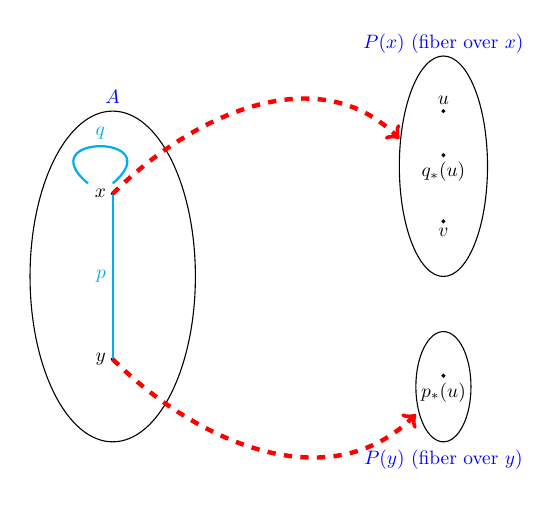
\begin{tikzpicture}[scale=0.7,every node/.style={scale=0.7}]]
  \draw (-3,0) ellipse (1.5cm and 3cm);
  \draw (3,2) ellipse (0.8cm and 2cm);
  \draw (3,-2) ellipse (0.5cm and 1cm);
  \node[blue,ultra thick,above] at (-3,3) {$A$};
  \node[blue,ultra thick,above] at (3,3.9) {$P(x)$ (fiber over $x$)};
  \node[blue,ultra thick,below] at (3,-3) {$P(y)$ (fiber over $y$)};
  \draw[fill] (-3,1.5) circle [radius=0.025];
  \draw[fill] (-3,-1.5) circle [radius=0.025];
  \draw[left,cyan,thick] (-3,1.5) -- (-3,-1.5);
  \node[left] (X) at (-3,1.5) {$x$};
  \path[cyan,thick] (X) edge [loop above, looseness=8, in=40, out=140] node[above] {$q$} (X);
  \node[left] at (-3,-1.5) {$y$};
  \draw[fill] (3,-1.8) circle [radius=0.025];
  \draw[fill] (3,3) circle [radius=0.025];
  \node[above] at (3,3) {$u$};
  \draw[fill] (3,2.2) circle [radius=0.025];
  \node[below] at (3,2.2) {$q_*(u)$};
  \draw[fill] (3,1) circle [radius=0.025];
  \node[below] at (3,1) {$v$};
  \node[below] at (3,-1.8) {$p_*(u)$};
  \node[left,cyan] at (-3,0) {$p$};
  \draw[->,red,dashed,ultra thick] (-3,1.5) to [out=45, in=135] (2.2,2.5);
  \draw[->,red,dashed,ultra thick] (-3,-1.5) to [out=-45, in=-135] (2.5,-2.5);
\end{tikzpicture}
\end{center}

\noindent It is worth repeating Remark 2.7.1 from the book. In the figure above,
we could have $(x,u) \equiv (x,v)$ without necessarily having $u \equiv v$. The
only thing we can conclude regarding $u$ and $v$ is that there is a (possibly
non-trivial) path $q : x \equiv x$ such that $q_*(u) \equiv v$.

\paragraph*{Propositional Truncation.} Given a type $A : \mathcal{U}$, the type
$\|A\|$ is the propositional truncation of $A$ defined as follows: for
  any $x:A$ we have $|x| : \|A\|$, and for any $x,y : \|A\|$, we have
  $\gluep : x \equiv y$.

\paragraph*{Univalent Type Family.}
For each fibration, we have a function:
\[\begin{array}{rcl}
\textit {transport-equiv} &:& \Pi_{(P : A \to \mathcal{U})}~ \Pi_{(x,y:A)}~
    x \equiv y  \to P(x) \simeq P(y) \\
\textit{transport-equiv}~P~x~y &=& \lambda p. \mathit{idtoeqv}(\mathit{ap}_{P}(p))
\end{array}\]
We say a type family $P : A \to \mathcal{U}$ is \emph{univalent} if for all
$x,y:A$ the function $\textit{transport-equiv}~P~x~y$ is an
equivalence. Formally:
\[\begin{array}{l}
\textit{is-univalent-fibration} : (A \to \mathcal{U}) \to \mathcal{U} \\
\textit{is-univalent-fibration}~P = \Pi_{(x,y:A)} \textit{isequiv}~(\textit{transport-equiv}~P~x~y)
\end{array}\]

%%%%%
\subsection{Examples}

We will choose particular base spaces $A$ and fibrations $P : A \to \mathcal{U}$
below and reason about whether they are univalent or not. For each fibration,
the question of whether it is univalent reduces to whether, for all $x,y:A$, the
function $\textit{transport-equiv}~P~x~y$ is an equivalence. In other words, the
question we are asking is whether we have an equivalence
$(x \equiv y) \simeq (P(x) \simeq P(y))$ witnessed by the function
$\textit{transport-equiv}~P~x~y$.

\begin{itemize}

\item Take $A = \mathcal{U}$ and $P = \mathit{Id}_{\mathcal{U}}$. By definition,
  this fibration is univalent if
  $\textit{transport-equiv}~\mathit{Id}_{\mathcal{U}}~x~y = \mathit{idtoeqv}$ of
    type $x \equiv y \to x \simeq y$ is an equivalence. As Axiom 2.10.3 in the
    book states this is exactly the statement of the conventional univalence
    axiom for universe $\mathcal{U}$.

\item Take $A = \ot$ with element $\star$ and $P = \lambda \_. \ot$. This
    fibration $P$ is univalent if we have an equivalence
    $(\star\equiv\star) \simeq (\ot\simeq\ot)$ witnessed by
    $\textit{transport-equiv}~P~x~y$. The two types are clearly equivalent in
    this case.

\item Take $A = \ot$ and $P = \lambda \_. \zt$. This fibration is univalent if
    we have an equivalence $(\star\equiv\star)\simeq(\zt\simeq\zt)$ witnessed by
    $\textit{transport-equiv}~P~x~y$. The two types are also clearly equivalent
    in this case.

\item Take $A = \ot$. For no $P$ other than the above two instances will we
    have a univalent fibration.

\item Take $A = \bt$ with elements $\fc$ and $\tc$ and
  $P = \lambda \_. \ot$. The statement
  $\textit{is-univalent-fibration}~P$ reduces to $(\fc \equiv \tc) \simeq
  (\ot\simeq\ot)$ which is false.

\item Take $A = \bt$ with elements $\fc$ and $\tc$ and
  $P = \lambda \{ \fc \to \zt; \tc \to \ot \}$. This fibration is univalent if
  we have an equivalence $(\fc \equiv \tc) \simeq (\zt\simeq\ot)$ which is
  true. That is the only choice of $P$ that works (modulo symmetry).

\item For any $n > 2$, taking $A$ as sum of $n$ copies of $\ot$ can never
  give a univalent fibration.

\item For any type $F$ we define
  $\{F\} = \Sigma_{(A : \mathcal{U})} \| F \simeq A \|$. By a proposition of
  Christensen, any fibration with base space $\{F\}$, i.e., any fibration
  $\{F\} \to \mathcal{U}$, is univalent. In particular, we can take the base
  space to be:
  \begin{itemize}
  \item $\{\ot\}$. The type $\{\ot\}$ is actually the same as $\ot$ and this was
    covered by previous examples.
  \item $\{S^1\}$. The type $\{S^1\}$ is the same as $S^1$. This is perhaps the
    simplest base space to choose but it does not naturally correspond to a
    conventional programming language.
  \item $\{\bt\}$. In some sense this is the simplest
    programming-language--relevant universe --- our featherweight HoTT. We aim
    to characterize this base space as a reversible programming language based
    on type isomorphisms.
  \end{itemize}

\end{itemize}

%%%%%%%%%%%%%%%%%%%%%%%%%%%%%%%%%%%%%%%%%%%%%%%%%%%%%%%%%%%%%%%%%%%%%%%%%%%%%%
\section{Analyzing $\{\bt\}$ and its Connection to $\Pi$}

%%%%%
\subsection{The Subuniverse $\{\bt\}$}

\textbf{Theorem.} For any type $F$, the type $\Sigma_{A:\mathcal{U}} \| F \equiv A \|$ is the base
of a univalent fibration.


Recall that
$\{\bt\} = \Sigma_{(A:\mathcal{U})} \|A \simeq \bt\| = \Sigma_{(A:\mathcal{U})}
\| \mathit{Bool} \equiv A\|$. We begin by unpacking the objects, 1-paths, and 2-paths of
$\{\bt\}$.

\paragraph*{Objects in $\{\bt\}$.} The only term in $\{\bt\}$ is
$(\bt,\|\reflp_{\bt}\|)$ which we call $`\bt$. Formally we can prove
$\|(X,p) \equiv `\bt\|$ is inhabited for all $X$ and $p$.

\paragraph*{1-Paths in $\{\bt\}$.} These are paths between $`\bt$ and
$`\bt$. Generally speaking, paths between elements of a $\Sigma$-type are pairs
of paths with a transport in the second component. If we have a type $A$ with
points $a$ and $b$ and a path $p : a \equiv b$. Fix some $c$ and consider the
dependent function $(x:A) \rightarrow (x \equiv c)$. This forms the types
$a\equiv c$ and $b\equiv c$ with elements $ua$ and $ub$. Now a path between
$(a,ua)$ and $(b,ub)$ is a pair $(p,\alpha)$ where $\alpha : p_* ua \equiv
ub$. Hence paths between $`\bt$ and $`\bt$ are going to be for the form
$(p,\alpha)$ where $p : \bt \equiv \bt$ and $\alpha$ is essentially $\gluep$
from the definition of truncation. So we have two paths:
\[\begin{array}{rcl}
`\mathbf{id} &=& (\reflp,\gluep) \\
`\mathbf{not} &=& (\notp,\gluep)
\end{array}\]

\paragraph*{2-Paths in $\{\bt\}$.} Now are considering paths between
$`\mathbf{id}$ and $`\mathbf{id}$, and between $`\mathbf{not}$ and
$`\mathbf{not}$. We have at least one path at this level which is
$(\reflp,\gluep)$ but to show that that this is the only path we will have to
first prove that $`\mathbf{not} \circ `\mathbf{not} \equiv `\mathbf{id}$.



%%%%%
\subsection{Equivalence}

Now we claim that $\{\bt\}$ is equivalent to $\mathcal{U}_\Pi$ which is the
universe which includes types $\tau$ as a points, combinators
$c : \tau_1 \iso \tau_2$ as 1-paths, and 2-combinators
$\alpha : c_1 \isotwo c_2$ as 2-paths. The proof is in a meta-logic which is
itself univalent.

%%%%%%%%%%%%%%%%%%%%%%%%%%%%%%%%%%%%%%%%%%%%%%%%%%%%%%%%%%%%%%%%%%%%%
%%%%%%%%%
\section{Generalization I}

Use all finite types instead of just Bool

%%%%%%%%%%%%%%%%%%%%%%%%%%%%%%%%%%%%%%%%%%%%%%%%%%%%%%%%%%%%%%%%%%%%%
%%%%%%%%%
\section{Generalization II}

Add a HIT to the univalent universe, perhaps something to do with fractionals.

%%%%%%%%%%%%%%%%%%%%%%%%%%%%%%%%%%%%%%%%%%%%%%%%%%%%%%%%%%%%%%%%%%%%%%%%%%%%%%
\bibliographystyle{acm}
{\footnotesize
\bibliography{cites}
}
\end{document}
